\chapter{Sound}

When you set off a firecracker, it makes sound.

Let's break that down a little more: Inside the cardboard wrapper of
the firecracker, there is potassium nitrate ($KNO_3$), sulfer ($S$),
and carbon($C$).  These are all solids. When you trigger the chemical
reactions with a little heat, these atoms rearrange themselves to be
potassium carbonate ($K_2CO_3$), potassium sulfate ($K_2SO_4$), carbon
dioxide ($CO_2$), and nitrogen ($N_2$). Note that the last two are
gasses.

The molecules of a solid are much more tightly packed than the
molecules of a gas. So after the chemical reaction, the molecules
expand to fill a much bigger volume. The air molecules nearby get
pushed away from the firecracker.  They compress the molecules beyond
them, and those compress the molecules beyond them.

This compression wave radiates out as a sphere; its radius growing at
about 343 meters per second (``The speed of sound'').

The energy of the explosion is distributed around the surface of this
sphere. As the radius increases, the energy is spread more and more
thinly around. This is why the firecracker seems louder when you are
closer to it. (If you set off a firecracker in a sewer pipe, the sound
will travel much, much farther.)

This compression wave will bounce off of hard surfaces. If you set off
a firecracker 50 meters from a big wall, you will hear the explosion
twice. We call the second one ``an echo.''

The compression wave will be absorbed by soft surfaces. If you covered
that wall with pillows, there would be almost no echo.

The study of how these compression waves move and bounce is called
\newterm{accoustics}. Before you build a concert hall, you hire an
accoustician to look at your plans and tell you how to make it sound
better.

\section{Pitch and frequency}

The string on a guitar is very similar to the weighted spring
example. The farther the string is displaced, the more force it feels
pushing it back to equilibrium. Thus, it moves back and forth in a
sine wave. (OK, it isn't a pure sine wave, but we will get to that later.)

The string is connected to the center of the boxy part of the guitar,
which is pushed and pulled by the string. That creates compression
waves in the air around it.

If you are in the room with the guitar, those compression waves enter
your ear, push and pull your ear drum, which is attached to bones that
move a fluid that tickles tiny hairs, called \newterm{cilia} in your
inner ear. That is how you hear.

We sometimes see plots of sound waveforms.  The $x$-axis represents
time. The $y$-axis represents the amount the air is compressed at the
microphone that converted the air pressure into an electrical signal.

\includegraphics[width=0.8\linewidth]{soundwave.png}

If the guitar string is made tighter (by the tuning pegs) or shorter
(by the guitarist's fingers on the strings), the string vibrates more
times per second.  We measure the number of waves per second and we
call it the \newterm{frequency} of the tone. The unit for frequency is
\newterm{Hertz}: cycles per second.

Musicans have given the different frequencies names. If the guitarist
plucks the lowest note on his guitar, it will vibrate at 82.4
Hertz. The guitarist will say ``That pitch is low E.'' If the string is made
half as long (by a finger on the 12th fret), the frequency will be
twice as fast (164.8 Hertz), and the guitarist will say ``That is E an
octave up.''

For any note, the note that has twice the frequency is one octave
up. The note that has half the frequency is one octave down.

The octave is a very big jump in pitch, so musicians break it up into
12 smaller steps. If the guitarist shortens the E string by one fret,
the frequency will be $82.4 \times 1.059463 \approx 87.3$ Hertz. 

Shortening the string one fret always increases the frequency by a factor of 1.059463. Why?

Because $1.059463^12 = 2$. That is, if you take 12 of these hops, you
end up an octave higher.

This, the smallest hop in western music, is referred to as \newterm{half step}.

\begin{Exercise}[title={Notes and frequecies}, label=note_to_frequency]

The note A near the middle of the piano, is 440Hz. The note E is 7 half steps above A.  What is its frequency?
 
\end{Exercise}
\begin{Answer}[ref=note_to_frequency]

  A is 440 Hz.  Each half-step is a multiplication by $\sqrt[12]{2} = 1.059463094359295$
  So the frequency of E is $(440)(2^{7/12}) = 659.255113825739859$

\end{Answer}


\section{Chords and harmonics}

Of course, a guitarist seldom plays only one string at a
time. Instead, he uses the frets to pick a pitch for each string and
strums all six strings.

Some combinations of frequencies sound better than others. We have
already talked about the octave: if one string vibrates twice for each
vibration of another, they sound sweet together.

Musicians speak of ``the fifth''.  If one string vibrates three times
and the other vibrates twice in the same amount of time, they sound
sweet together.

If one string vibrates 4 times while the other vibrates 3 times, they
sound sweet together. Musicians call this ``the third.''

Each of these different frequencies tickle different cilia in the
inner ear, so you are able to hear all six notes at the same time when
the guitarist strums his guitar.

When a string vibrates, it doesn't create a single sine wave. Yes, the
string vibrates from end-to-end and this generates a sine wave at what
we call \newterm{the fundmental frequency}.However, there are also
``standing waves'' on the string. One of these standing waves, is
still at the centerpoint of the string, but everything to the left of
the centerpoint is going up when everything to the right is going
down. This creates \newterm{an overtone} that is twice the frequency
of the fundamental.

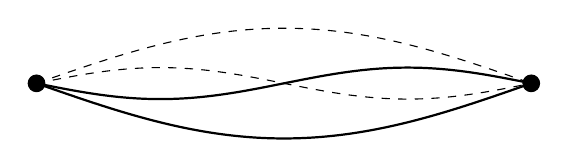
\begin{tikzpicture}[
tl/.style = {% tick labels
    fill=white, inner sep=1pt, font=\scriptsize,
            },                        ]

  \draw[dashed,draw=black,
      domain=-0:6.283,samples=300,variable=\x] 
      plot (\x,{0.7 * sin(deg{\x}/2)});
  \draw[thick,draw=black,
      domain=0:6.283,samples=300,variable=\x] 
  plot (\x,{0.7 * sin(deg{-1 * \x}/2)});
  
  \draw[dashed,draw=black,
      domain=-0:6.283,samples=300,variable=\x] 
      plot (\x,{0.2 * sin(deg{\x})});
  \draw[thick,draw=black,
      domain=0:6.283,samples=300,variable=\x] 
      plot (\x,{0.2 * sin(deg{-1 * \x})});

 \filldraw[black] (0, 0)  circle(3pt);
 \filldraw[black] (6.283, 0)  circle(3pt);

\end{tikzpicture}

The next overtone has two still points -- it divides the string into
three parts.  The outer parts are up while the inner part is
down. It's frequency is three times the fundamental frequency.

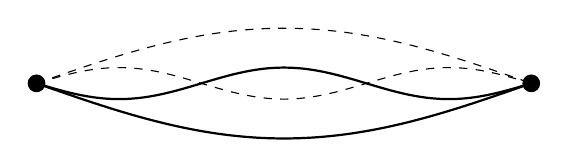
\begin{tikzpicture}[
tl/.style = {% tick labels
    fill=white, inner sep=1pt, font=\scriptsize,
            },                        ]

  \draw[dashed,draw=black,
      domain=-0:6.283,samples=300,variable=\x] 
      plot (\x,{0.7 * sin(deg{\x}/2)});
  \draw[thick,draw=black,
      domain=0:6.283,samples=300,variable=\x] 
  plot (\x,{0.7 * sin(deg{-1 * \x}/2)});
  
  \draw[dashed,draw=black,
      domain=-0:6.283,samples=300,variable=\x] 
      plot (\x,{0.2 * sin(1.5 * deg{\x})});
  \draw[thick,draw=black,
      domain=0:6.283,samples=300,variable=\x] 
      plot (\x,{0.2 * sin(1.5 * deg{-1 * \x})});

 \filldraw[black] (0, 0)  circle(3pt);
 \filldraw[black] (6.283, 0)  circle(3pt);

\end{tikzpicture}

And so on: 4 times the fundamental, 5 times the fundamental, etc.

In general, tones with a lot of overtones tend to sound bright. Tones
with just the fundamental sound thin.

Humans can generally hear frequencies from 20Hz to 20,000Hz (or
20kHz).  Young people tend to be able to hear very high sounds better
than older people.

Dogs can generally hear sounds in the 65Hz to 45kHz range.

\section{Making waves in Python}

Let's make a sine wave and add some overtones to it.  Create a file \filename{harmonics.py}

\begin{Verbatim}
import matplotlib.pyplot as plt
import math

# Constants: frequency and amplitude
fundamental_freq = 440.0 # A = 440 Hz
fundamental_amp = 2.0

# Up an octave
first_freq = fundamental_freq * 2.0 # Hz
first_amp = fundamental_amp * 0.5

# Up a fifth more
second_freq = fundamental_freq * 3.0 # Hz
second_amp = fundamental_amp * 0.4

# How much time to show
max_time = 0.0092 # seconds

# Calculate the values 10,000 times per second
time_step = 0.00001 # seconds

# Initialize 
time = 0.0
times = []
totals = []
fundamentals = []
firsts = []
seconds = []

while time <= max_time:
    # Store the time
    times.append(time)
    
    # Compute value each harmonic
    fundamental = fundamental_amp * math.sin(2.0 * math.pi * fundamental_freq * time)
    first = first_amp * math.sin(2.0 * math.pi * first_freq * time)
    second = second_amp * math.sin(2.0 * math.pi * second_freq * time)

    # Sum them up
    total = fundamental + first + second

    # Store the values
    fundamentals.append(fundamental)
    firsts.append(first)
    seconds.append(second)
    totals.append(total)

    # Increment time
    time += time_step

# Plot the data
fig, ax = plt.subplots(2, 1)

# Show each component
ax[0].plot(times, fundamentals)
ax[0].plot(times, firsts)
ax[0].plot(times, seconds)
ax[0].legend()

# Show the totals
ax[1].plot(times, totals)
ax[1].set_xlabel("Time (s)")

plt.show()
\end{Verbatim}

When you run it, you should see a plot of all three sine waves and another plot of their sum:

\includegraphics[width=0.9\linewidth]{harmonicspy.png}

\subsection{Making a sound file}

The graph is pretty to look at, but make a file that we can listen to.

The WAV audio file format is supported on pretty much any device, and
a library for writing WAV files comes with Python.  Lets write some
sine waves and some noise into a WAV file.

Create a file called \filename{soundmaker.py}

\begin{Verbatim}
import wave
import math
import random

# Constants
frame_rate = 16000 # samples per second
duration_per = 0.3 # seconds per sound
frequencies = [220, 440, 880, 392] # Hz
amplitudes = [20, 125]
baseline = 127 # Values will be between 0 and 255, so 127 is the baseline
samples_per = int(frame_rate * duration_per) # number of samples per sound

# Open a file
wave_writer = wave.open('sound.wav', 'wb')

# Not stereo, just one channel
wave_writer.setnchannels(1)

# 1 byte audio means everything is in the range 0 to 255
wave_writer.setsampwidth(1)

# Set the frame rate
wave_writer.setframerate(frame_rate)

# Loop over the amplitudes and frequencies
for amplitude in amplitudes:
    for frequency in frequencies:
        time = 0.0
        # Write a sine wave
        for sample in range(samples_per):
            s = baseline + int(amplitude * math.sin(2.0 * math.pi * frequency * time))
            wave_writer.writeframes(bytes([s]))
            time += 1.0 / frame_rate
            
        # Write some noise after each sine wave
        for sample in range(samples_per):
            s = baseline + random.randint(0, 15)
            wave_writer.writeframes(bytes([s]))
            
# Close the file
wave_writer.close()
\end{Verbatim}

When you run it, it should create a sound file with several tones of
different frequencies and volumes. Each tone should be followed by
some noise.
